\documentclass{beamer}

\usepackage{amsmath}
\usepackage{tabularx}
\usepackage{amsfonts}       
\usepackage{amssymb}        
\usepackage{amsthm}         

\setbeamertemplate{caption}{\raggedright\insertcaption\par}

\title{Elliptic Curves}
\subtitle{Thesis Defense}
\institute{Tufts University}
\date{April 2017}
\subject{Mathematics}

\graphicspath{{images/}}

\newcommand{\Q}{\mathbb{Q}}
\newcommand{\F}{\mathbb{F}}
\newcommand{\Z}{\mathbb{Z}}


\begin{document}


\frame{\titlepage}

\begin{frame} 
\frametitle{Table of Contents} 
\tableofcontents
\end{frame}

\section{What is an elliptic curve?}

\begin{frame}
\frametitle{Definition}
An elliptic curve is a nonsingular 
cubic plane curve with at least one 
rational point.
\begin{figure}[H]
\begin{minipage}[b]{0.25\linewidth}
\centering

\includegraphics[width=\textwidth]{ch2-first-curves-1.png}
\caption{$y^2=x^3+x+1$}
\label{fig:a}
\end{minipage}
\hspace{0.5cm}
\begin{minipage}[b]{0.25\linewidth}
\centering

\includegraphics[width=\textwidth]{ch2-first-curves-2.png}
\caption{$y^2 = x^3 - x + 1$}
\label{fig:b}
\end{minipage}
\hspace{0.5cm}
\begin{minipage}[b]{0.25\linewidth}
\centering
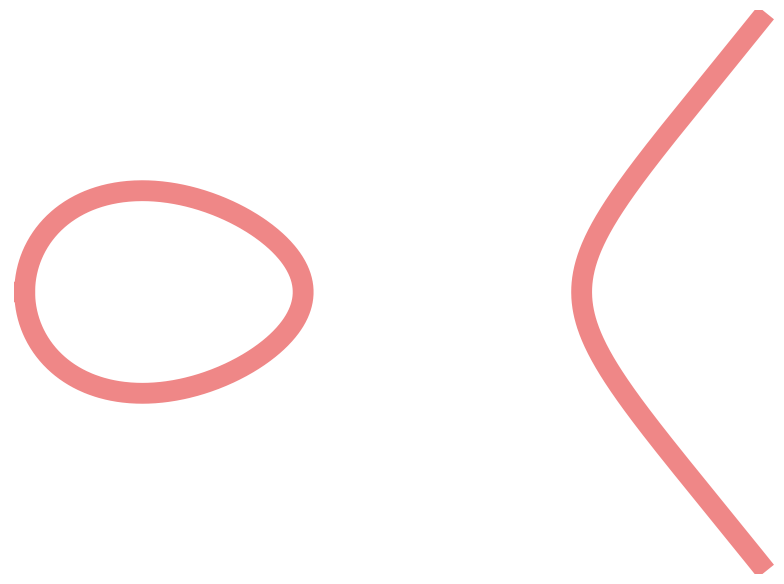
\includegraphics[width=\textwidth]{ch2-first-curves-3.png}
\caption{$y^2 = x^3 - x$}
\label{fig:b}
\end{minipage}
\end{figure}
\end{frame}

\begin{frame}
\frametitle{Singular Curves}
\begin{figure}[H]
\begin{minipage}[b]{0.25\linewidth}
\centering

\includegraphics[width=\textwidth]{ch2-singular-node.png}
\caption{Crunode: $y^2=x^3+x^2$}
\label{fig:a}
\end{minipage}
\hspace{0.5cm}
\begin{minipage}[b]{0.25\linewidth}
\centering

\includegraphics[width=\textwidth]{ch2-singular-cusp.png}
\caption{Ordinary Cusp: $y^2=x^3$}
\label{fig:b}
\end{minipage}
\hspace{0.5cm}
\begin{minipage}[b]{0.25\linewidth}
\centering

\includegraphics[width=\textwidth]{ch2-acnode.png}
\caption{Acnode: $y^2 = x^3 - x^2$}
\label{fig:b}
\end{minipage}
\end{figure}
\end{frame}

\section{History}
\begin{frame}
\frametitle{Timeline}
{\scriptsize
{\linespread{1}
\begin{table}[htbp]
\centering
\label{tbl:1}
\begin{tabular}{r l}
\hline
~285 a.d.  & Diophantus publishes \textit{Arithmetica} \\
...  & \\
1637 & Fermat states Fermat's Last Theorem \\
1669 & Newton expresses arc-lenghts of ellipses as infinite series  \\
1750 & Euler states a group law for Elliptic Integrals  \\
1779 & Bezout's Theorem is Stated  \\
...  & Gauss, Fagnano, Bernoulli, Legendre, Jacobi, Eisenstein, Abel,  \\
& and others work on elliptic functions  \\
1862 & Weierstra{\ss} Parametrizes $\wp$  \\
1916 & Ramanujan conjectures $\tau$ congruences  \\
1922 & Mordell's Theorem  \\
1928 & Mordell-Weil Theorem \\
1933 & Hasse's Bound  \\
1973 & Deligne Proves Weil's Riemann Hypothesis  \\
1977 & Mazur's Torsion Theorem  \\
1985 & Elliptic Curve Cryptography is born  \\
1987 & Lenstra's Integer Factorization Algorithm  \\
1995 & Wiles' Modularity Theorem  \\
2006 & Elkies' Discovery of a Rank $\geq$ 28 Curve  \\
2006 & Proof of the Sato-Tate Conjecture is Finished  \\
\hline
\end{tabular}
\end{table}
}}
\end{frame}

\section{Bezout's Theorem}
\begin{frame}
% https://terrytao.wordpress.com/tag/bezouts-theorem/
% http://math.mit.edu/~lguth/PolyMethod/lect13.pdf
% https://www.math.leidenuniv.nl/scripties/HulstBach.pdf
\frametitle{Bezout's Theorem in the Plane}
\begin{theorem}
Let $k$ be a field, and let $P, Q \in k[x,y]$ be non-zero 
polynomials in two variables $x,y$ with no common factor.
Then the two curves 
$\{ (x,y) \in k^2 \colon P(x,y) = 0 \}$ and 
$\{ (x,y) \in k^2 \colon Q(x,y) = 0 \}$ 
intersect at most 
$\text{deg}(P) \text{deg}(Q)$ times.
\end{theorem}
\begin{figure}[H]
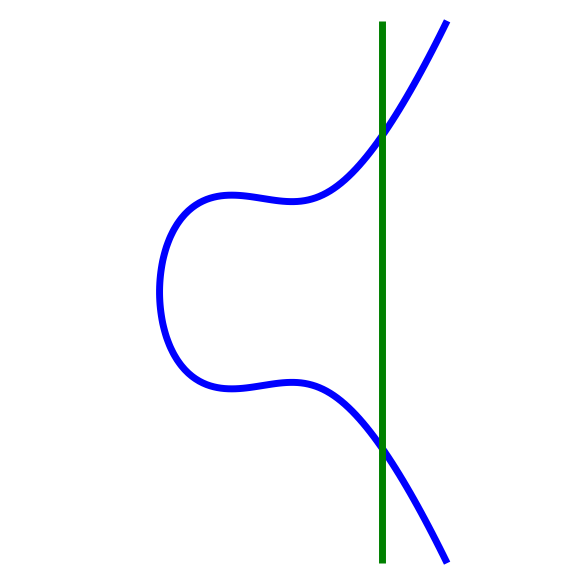
\includegraphics[width=.3\textwidth]{affine-intersection}
\caption{$y^2 = x^3 + x^2 + 1$ and $x=1$}
\end{figure}
\end{frame}

\begin{frame}
\frametitle{Projective Geometry}
$\mathbb A^2(k) = k^2$ and $\mathbb P^2(k) = \{ (x,y,z) \in k^3 \colon (x,y,z) \neq (0,0,0) \} / \sim$ 
where $\sim$ is the equivalence relation where $(x,y,z) \sim (x',y',z')$ if and only if there 
is a scaling factor $c \neq 0$ such that $(x,y,z) = (cx', cy', cz')$. 
 
\begin{figure}[H]
\begin{minipage}[b]{0.4\linewidth}
\centering
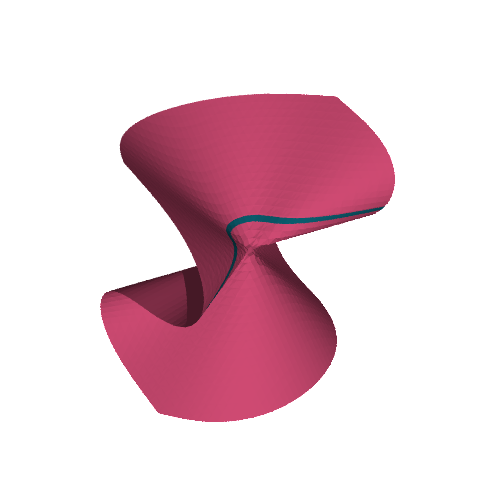
\includegraphics[width=\textwidth]{projective-elliptic-curve}
\label{fig:a}
\end{minipage}
\hspace{0.5cm}
\begin{minipage}[b]{0.4\linewidth}
\centering
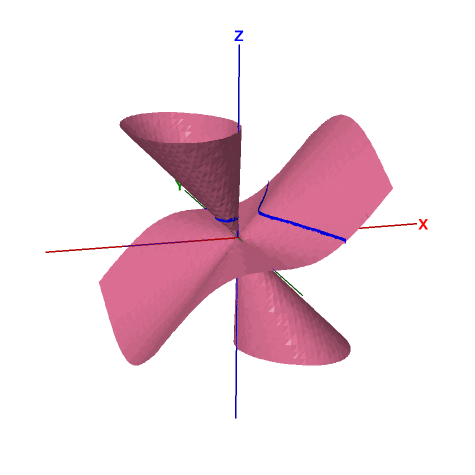
\includegraphics[width=\textwidth]{projective-elliptic-curve-2}
\label{fig:b}
\end{minipage}
\end{figure}
\end{frame}

\begin{frame}
\frametitle{Bezout's Theorem in Projective Geometry}
Let $P$ and $Q$ be homogeneous polynomials in the 
projective plane with no common factor. Then 
their projective solutions have 
$\text{deg}(P) \text{deg}(Q)$ intersection points 
counting multiplicity. 
\begin{figure}[H]
\centering
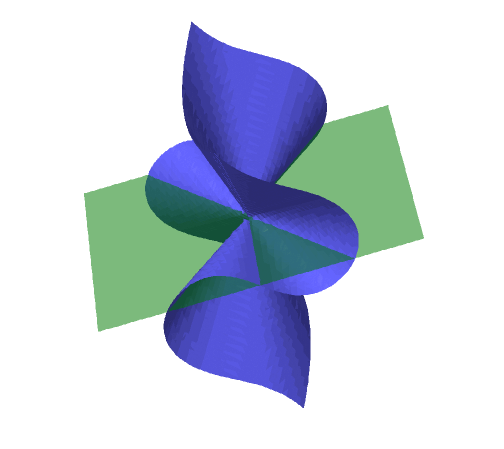
\includegraphics[width=.6\textwidth]{projective-intersection}
\caption{$y^2z = x^3 + x^2z + z^3$ and $x=z$}
\end{figure}
\end{frame}

\begin{frame}
\frametitle{Groups}
\begin{definition}
A group is a set $G$ with a binary operation $\cdot$ with the following properties
\begin{itemize}
\item[i.] There exists an identity, 1, such that $1\cdot g = g$ for every $g$ in $G$.
\item[ii.] Inverses exist for every element such that $g^{-1} g = gg^{-1} = 1$ for
every $g$ in $G$.
\item[iii.] Group operation associates $(a\cdot b) \cdot c = a \cdot (b \cdot c)$
for any $a,b,c \in G$.
\item[iv.] A group is abelian if $a \cdot b = b \cdot a$ for all $a,b \in G$.
\item[v.] A group is finitely generated if for some finite subset $S\subseteq G$ every
element in $G$ can be written as a group operation done unto elements of
$S$.
\end{itemize}
\end{definition}
\end{frame}

\section{Elliptic Curve Arithmetic}
\begin{frame}
\frametitle{Elliptic Curve Addition}
\begin{figure}[H]
\centering
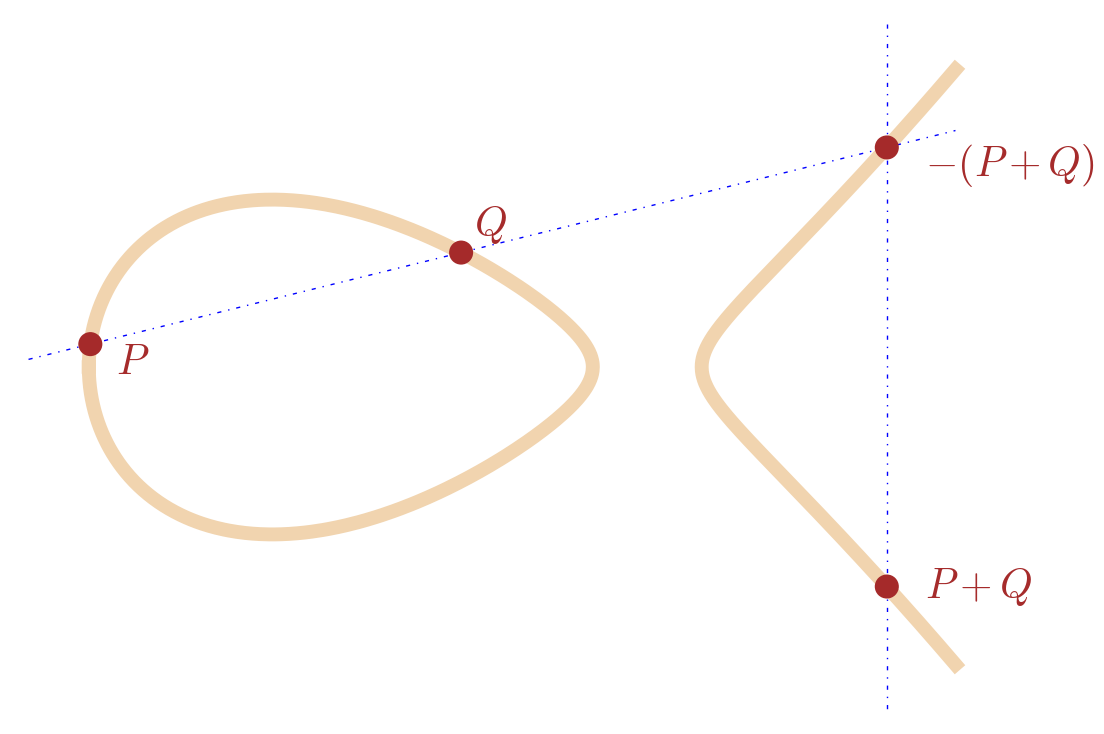
\includegraphics[width=\textwidth]{ch2-point-addition}
\end{figure}
\end{frame}

\begin{frame}
\frametitle{Elliptic Curve Multiplication (by $\mathbb Z$)}
\begin{figure}[H]
\centering
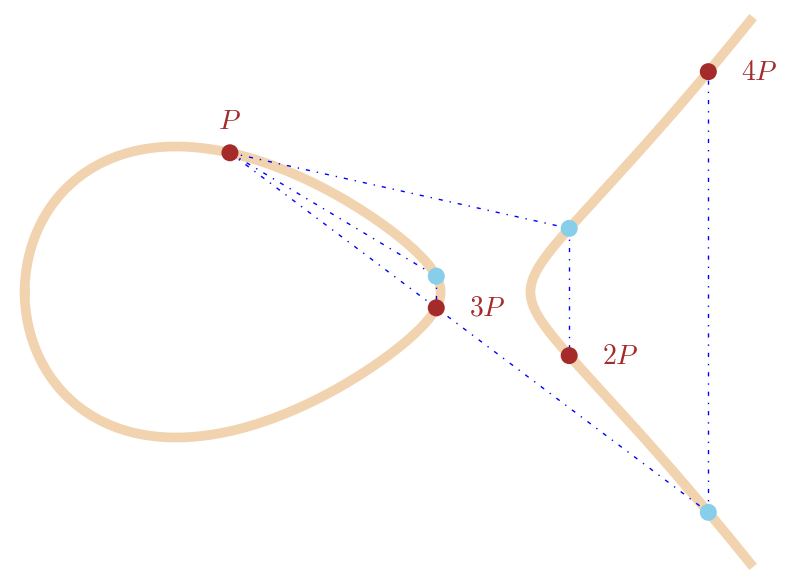
\includegraphics[width=\textwidth]{ch2-point-multiplication}
\end{figure}
\end{frame}


\section{Mordell's Theorem}
\begin{frame}
\frametitle{Mordell's Theorem}
The rational points of an elliptic curve are a finitely 
generated abelian group.
{\Large 
\[ E(\Q) = \underbrace{\Z + \Z + \cdots + \Z}_{r < \infty \text{ times}}  \hspace{.5cm} + \underbrace{\text{Torsion}}_{\text{a finite subgroup}} \]
}
\end{frame}

\begin{frame}
\frametitle{Mazur's Theorem}
% http://www.math.harvard.edu/theses/senior/schwartz/thesis.pdf
% http://www-personal.umich.edu/~asnowden/teaching/2013/679/
The torsion
subgroups of elliptic curves are the following fifteen groups.
\[ \mathbb Z / n \mathbb Z, \text{ where } 1 \leq n \leq 10 \text{ or } n = 12, \text{ or }\]
\[ \mathbb Z / 2 \mathbb Z \times \mathbb Z / n \mathbb Z, \text{ where }
n \in \{ 2, 4, 6, 8 \}. \]
\end{frame}

\begin{frame}
\frametitle{Finite Field Elliptic Curves}
\begin{figure}[H]
\centering
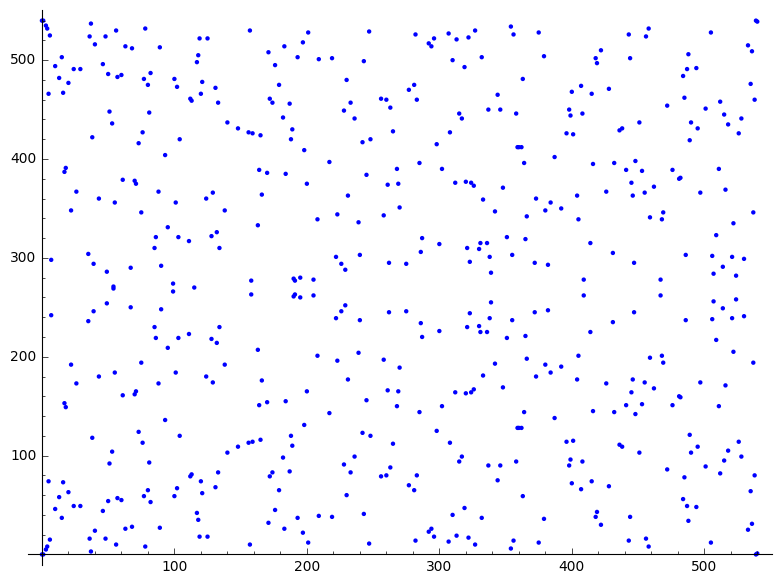
\includegraphics[width=.6\textwidth]{389a-finite-field-points}
\caption{$y^2 + y = x^{3} + x^{2} - 2 x$ over $\F_{541}$}
\end{figure}
\end{frame}

\section{Hasse's Bound}
\begin{frame}
\frametitle{Hasse's Bound}
Hasse showed the size of a finite 
field elliptic curve is bounded. 
\[ |E(\F_q)| - q - 1 \leq 2 \sqrt q. \]
\begin{figure}[H]
\begin{minipage}[b]{.45\linewidth}
\centering
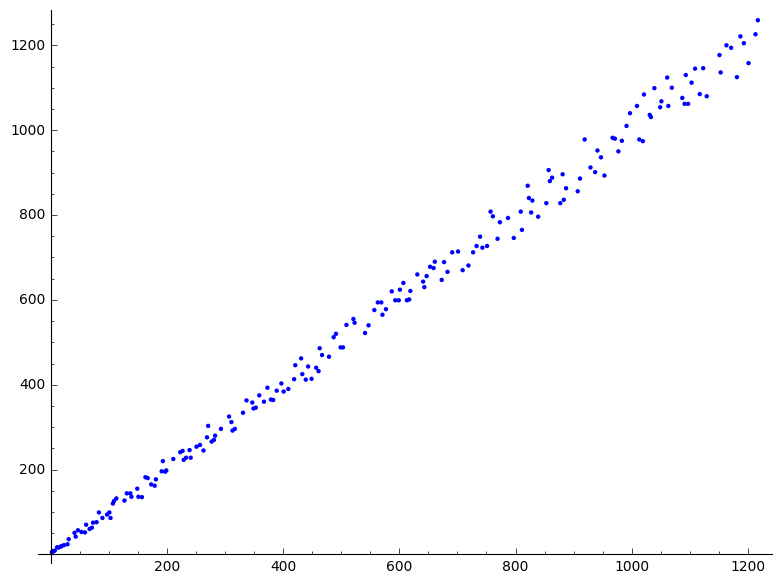
\includegraphics[width=\textwidth]{hasse-bound1}
\caption{$|E(\F_p)|$}
\end{minipage}
\hspace{.5cm}
\begin{minipage}[b]{.45\linewidth}
\centering
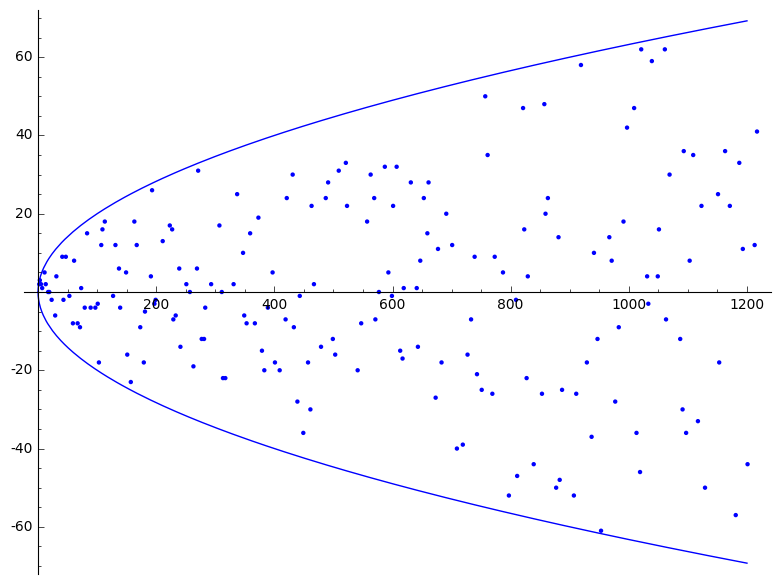
\includegraphics[width=\textwidth]{hasse-bound2}
\caption{$|E(\F_p)| - p - 1$}
\end{minipage}
\end{figure}
\end{frame}

\section{Lenstra's Factorization Algorithm}
\begin{frame}
\frametitle{Lenstra's Factorization Algorithm}
{\scriptsize
\begin{table}[htbp]
\centering
  \centering
  \begin{tabular}{|r l|}
  \hline
  \textbf{0.} & Let $n \geq 2$ be a composite integer to be factored. \\
  \textbf{1.} & Check that $\gcd(n,6) = 1$ and that $n$ is not a perfect power. \\
  \textbf{2.} & Choose random integers $b,$ $x_1$, and $y_1$ modulo $n$. \\
  \textbf{3.} & Set $P = (x_1,y_1)$ and $c = y_1^2 - x_1^3 - bx_1 \pmod n$. \\
  \textbf{4.} & Let $E$ be the elliptic curve $E : y^2 = x^3 + bx + c$. \\
  \textbf{5.} & Repeat Step 6 through 9 for $d = 2,3,4,\hdots$ up to a specified bound. \\
  \textbf{6.} & \hspace{.25in} Compute $Q = dP \pmod n$ and set $P = Q$. \\
   \textbf{7.} & \hspace{.25in} If the computation of Step 6 fails then we have found a divisor, \\
   & \hspace{.25in} $g = \gcd(x(Q) - x(P), n)$. \\
  \textbf{8.} & \hspace{.25in} If $g < n$, then we find $g$ is a factor of $n$. \\
  \textbf{9.} & \hspace{.25in} If $g = n$, go back to step 2 and pick a different curve and point. \\
  \textbf{10.} & If all factors have not yet been found, go back to step 2 and try again.\\
  \hline
  \end{tabular}
\end{table}
}
\end{frame}

\section{Experiments}
\begin{frame}
\frametitle{How Does $E(\Q)$ Reduce into $E(\F_p)$}
\[ F_E(p) = \frac{\displaystyle\sum_{\text{primes}\leq p}|\langle \text{free-generators}(E(\Q)) \rangle|}{\displaystyle\sum_{\text{primes} \leq p} |E(\F_p)|}\] 
\end{frame}

\begin{frame}
\frametitle{How Does $E(\Q)$ Reduce into $E(\F_p)$}
\begin{figure}[H]
\centering
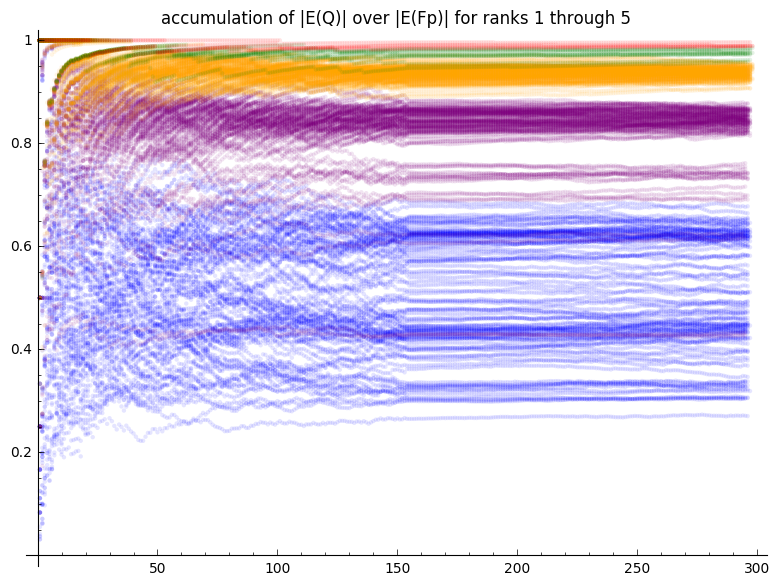
\includegraphics[width=.8\textwidth]{accumulation_index_huge}
\end{figure}
\end{frame}

\begin{frame}
\frametitle{How Does $E(\Q)$ Reduce into $E(\F_p)$}
\begin{figure}[H]
\centering
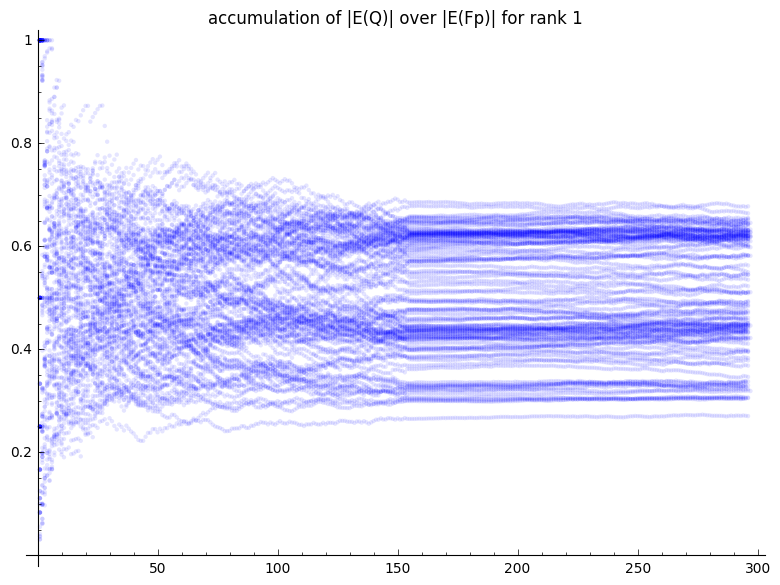
\includegraphics[width=.8\textwidth]{accumulation_index_1}
\end{figure}
\end{frame}

\begin{frame}
\frametitle{How Does $E(\Q)$ Reduce into $E(\F_p)$}
\begin{figure}[H]
\centering
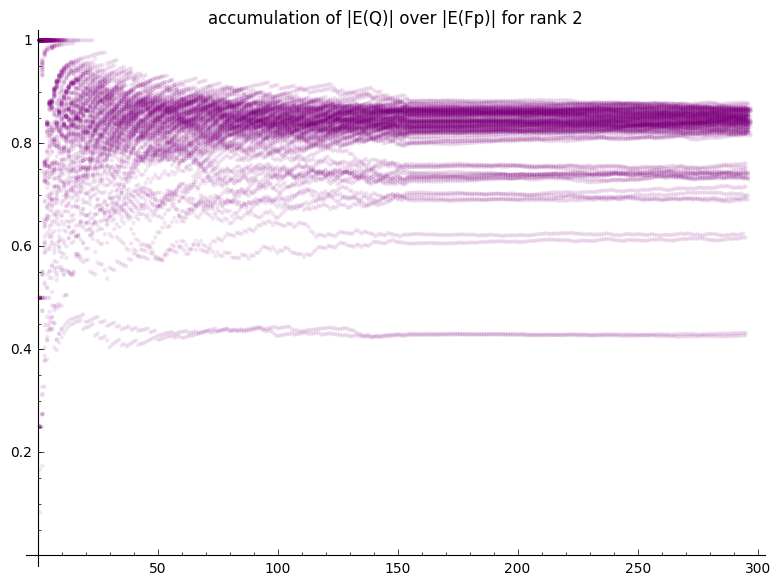
\includegraphics[width=.8\textwidth]{accumulation_index_2}
\end{figure}
\end{frame}

\begin{frame}
\frametitle{How Does $E(\Q)$ Reduce into $E(\F_p)$}
\begin{figure}[H]
\centering
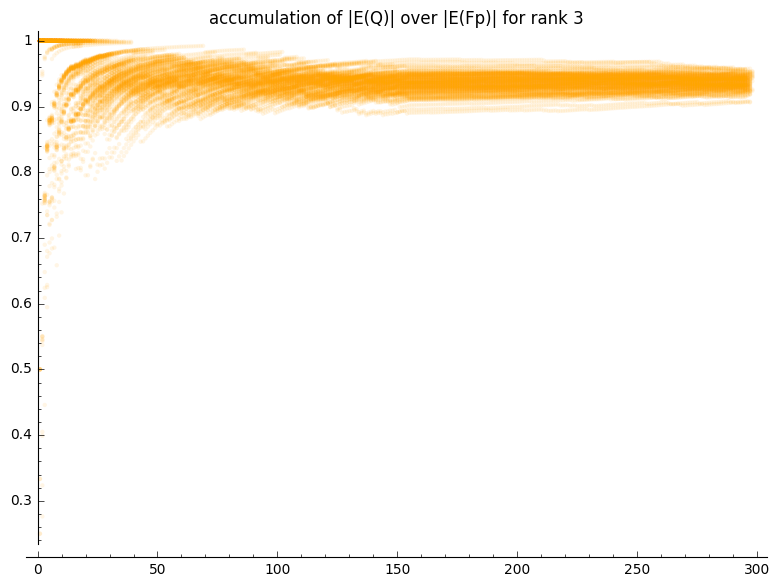
\includegraphics[width=.8\textwidth]{accumulation_index_3}
\end{figure}
\end{frame}

\begin{frame}
\frametitle{How Does $E(\Q)$ Reduce into $E(\F_p)$}
\begin{figure}[H]
\centering
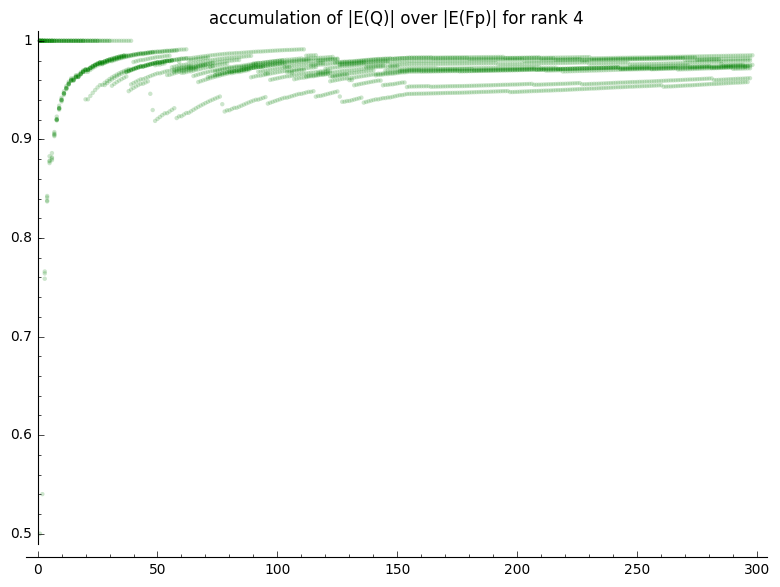
\includegraphics[width=.8\textwidth]{accumulation_index_4}
\end{figure}
\end{frame}

\begin{frame}
\frametitle{How Does $E(\Q)$ Reduce into $E(\F_p)$}
\begin{figure}[H]
\centering
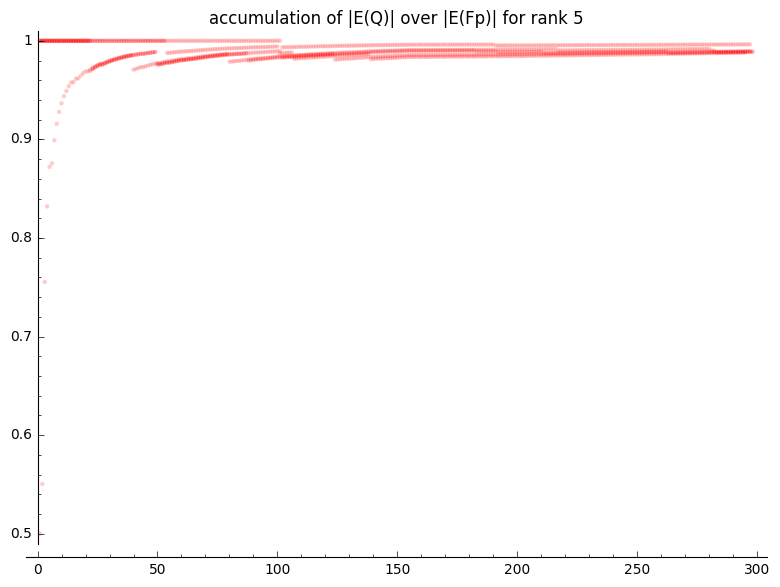
\includegraphics[width=.8\textwidth]{accumulation_index_5}
\end{figure}
\end{frame}

\begin{frame}
\frametitle{How Does $E(\Q)$ Reduce into $E(\F_p)$}
\begin{figure}[H]
\centering
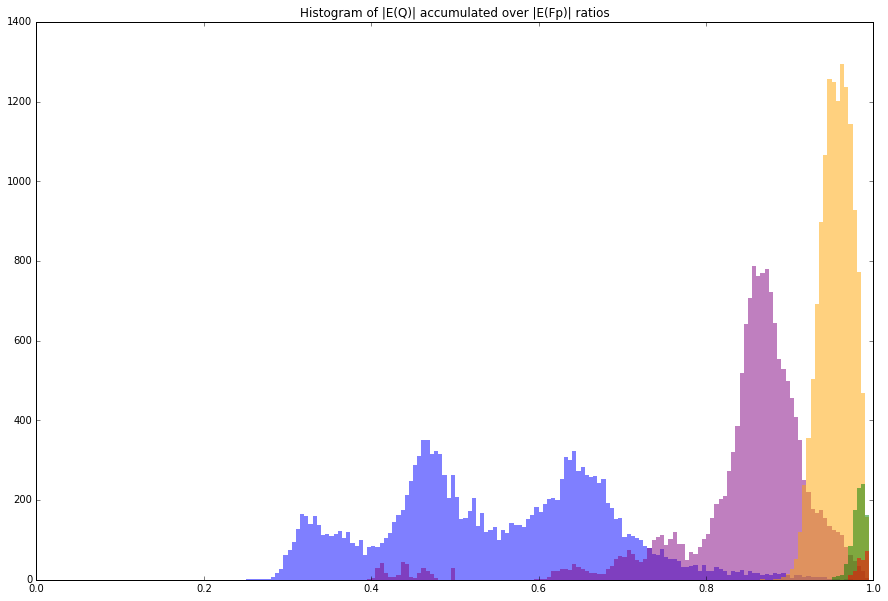
\includegraphics[width=.8\textwidth]{accumulation_hist_huge}
\end{figure}
\end{frame}


\begin{frame}
\frametitle{Generating a Subgroup with $(0,0)$}
Check it out! (0,0) is always on 
\[ E_{A,B} \colon y^2 + y = x^3 + Ax^2 + Bx \]
\end{frame}

\begin{frame}
\frametitle{Generating a Subgroup with $(0,0)$}
We define a set for each prime of elliptic 
curves 
\[ S_p = \{ E_{A,B} \colon \Delta(E) \neq 0 \text{ and } A,B \in \F_p \}. \]

And we define the following functions at each 
prime as a sum over this set. 
\[ F_1(p) = \displaystyle\sum_{E \in S_p} |E(\F_p)|, \]
\[ F_2(p) = \displaystyle\sum_{E \in S_p} |\langle (0,0) \rangle|, \]
\[ F_3(p) = \displaystyle\sum_{E \in S_p} [E(\F_p) : \langle (0,0) \rangle]. \]
\end{frame}

\begin{frame}
\frametitle{Generating a Subgroup with $(0,0)$}
\begin{figure}[H]
\centering
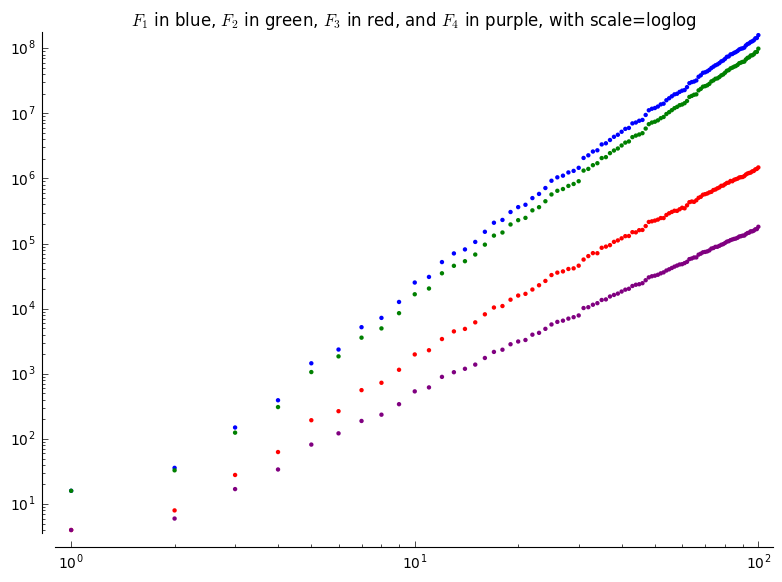
\includegraphics[width=.8\textwidth]{f_family}
\end{figure}
\end{frame}

\begin{frame}
\frametitle{Generating a Subgroup with $(0,0)$}
\begin{figure}[H]
\centering
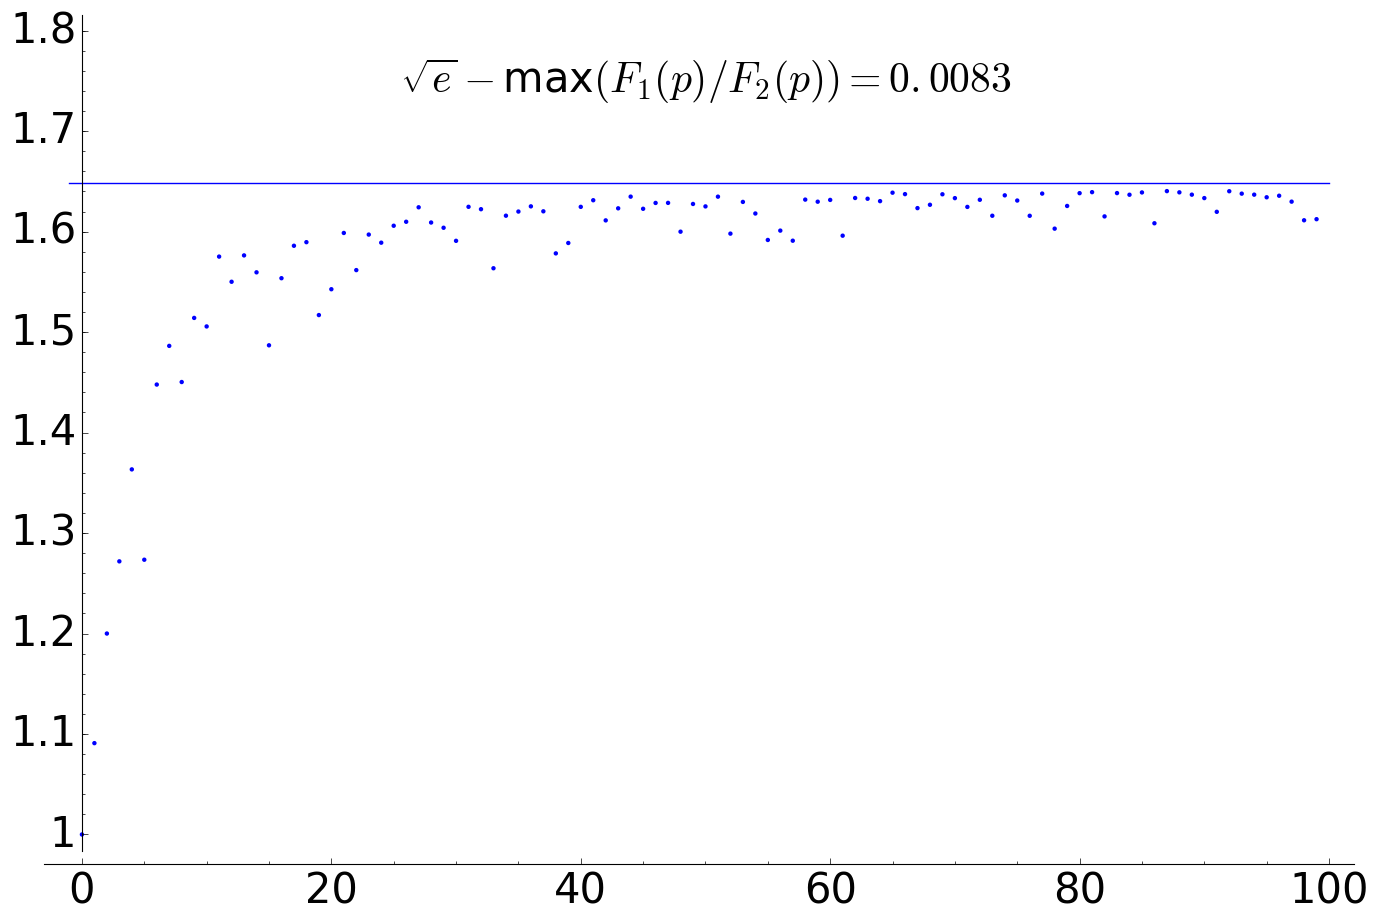
\includegraphics[width=.9\textwidth]{f1_div_f2}
\end{figure}
\end{frame}

\begin{frame}
\frametitle{Generating a Subgroup with $(0,0)$}
\begin{figure}[H]
\centering
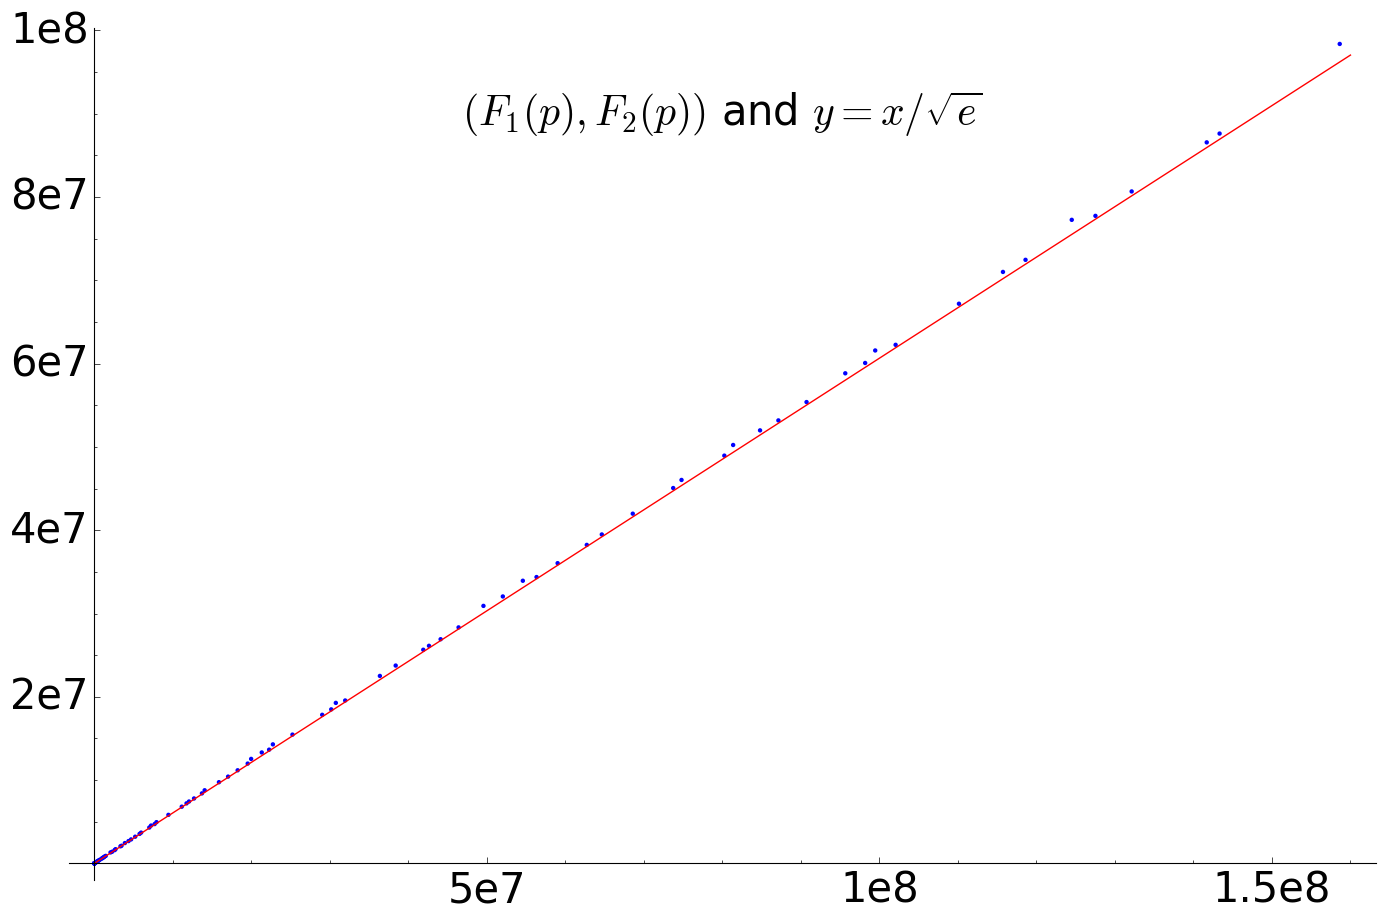
\includegraphics[width=.8\textwidth]{f1_f2_plot_bounded_by_sqrt_e}
\end{figure}
\end{frame}

\begin{frame}
\frametitle{Generating a Subgroup with $(0,0)$}
\begin{figure}[H]
\centering
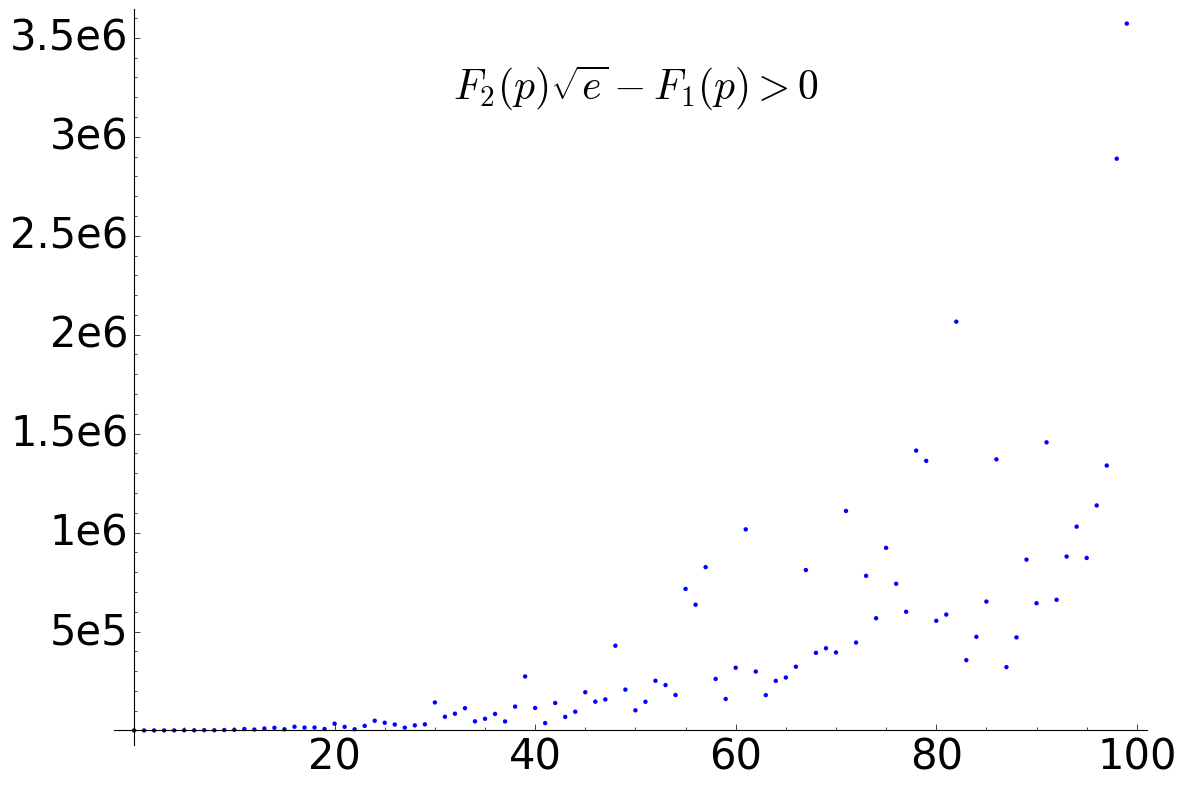
\includegraphics[width=.8\textwidth]{sqrt_e_error}
\end{figure}
\end{frame}


\begin{frame}
\frametitle{How Often is the Subgroup the Group?}
Now, we're investigating the 
divisibility of the index $[E(\F_p) : \langle (0,0) \rangle] = |E(\F_p)| / |\langle (0,0) \rangle|$. \\

How often is it one? How often is it even? How often is it divisible by $n$? 
\end{frame}

\begin{frame}
\frametitle{How Often is the Subgroup the Group?}
How often is $\frac{|E(F_p)|}{|\langle (0,0) \rangle|}$ one? About 44\% of the time.
\begin{figure}[H]
\centering
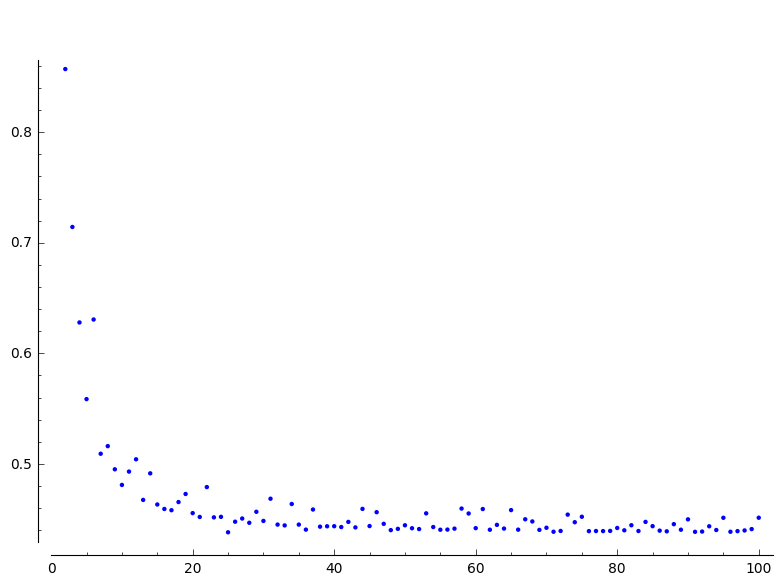
\includegraphics[width=.8\textwidth]{surjectivity_probability}
\end{figure}
\end{frame}

\begin{frame}
\frametitle{How Often is the Index Even?}
We believe that it's $10/24$ probability in the limit. 
\begin{figure}[H]
\centering
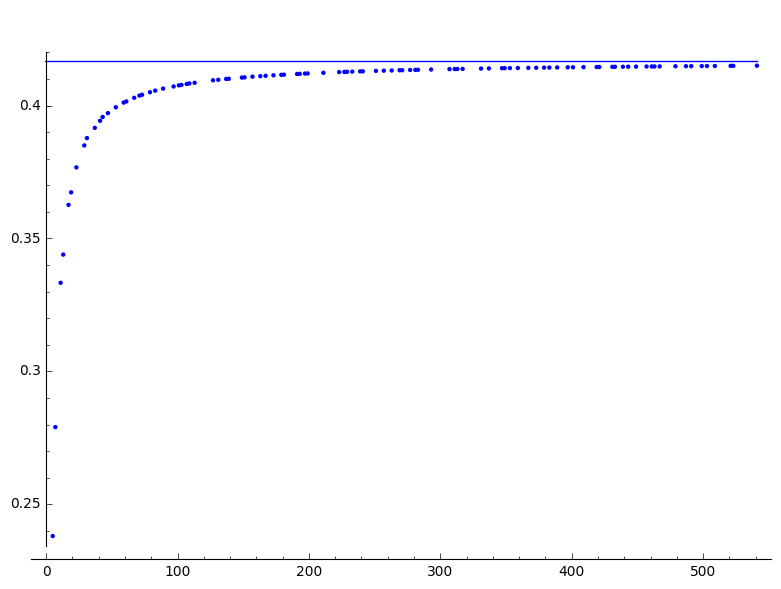
\includegraphics[width=.8\textwidth]{divisibility_two}
\end{figure}
\end{frame}

\begin{frame}
\frametitle{How Often is the Index Three Divisible?}
If $p = 1 \pmod p$, then the probability is $33/216$. \\
If $p = 2 \pmod p$, then the probability is $36/216$.
\begin{figure}[H]
\centering
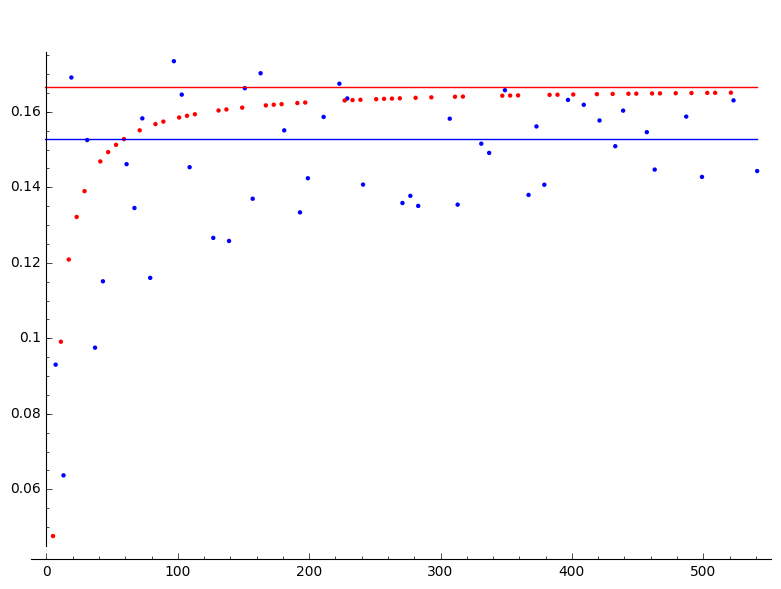
\includegraphics[width=.8\textwidth]{divisibility_three}
\end{figure}
\end{frame}

\begin{frame}
\frametitle{Error Analysis}
For our claim that 10/24 is the probability the 
index is even in the limit, we find that error 
from our conjectural bound decays exponentially.
\begin{figure}[H]
\centering
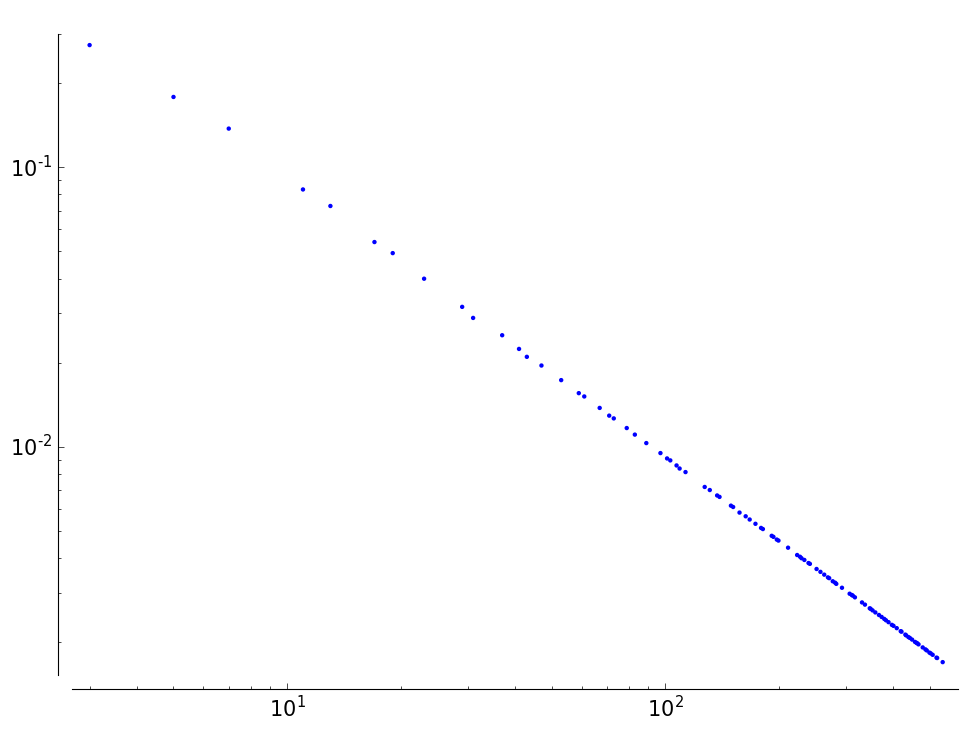
\includegraphics[width=.8\textwidth]{divisibility_claim_1}
\end{figure}
\end{frame}

\begin{frame}
\frametitle{Error Analysis}
And a similar story for 36/216
\begin{figure}[H]
\centering
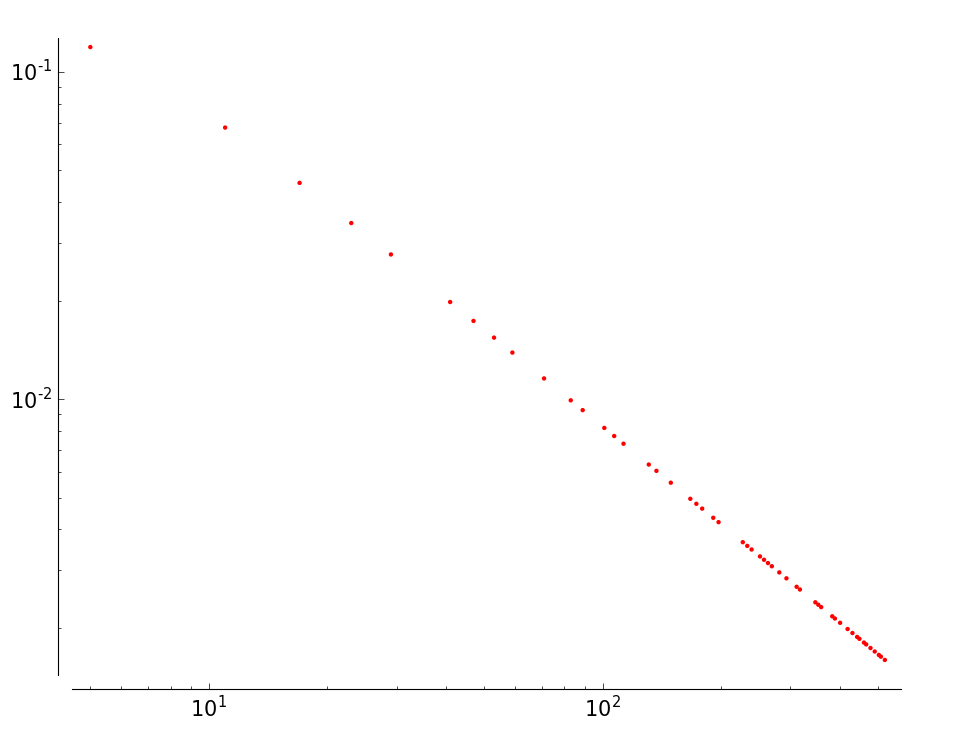
\includegraphics[width=.8\textwidth]{divisibility_claim_2}
\end{figure}
\end{frame}

\begin{frame}
\begin{figure}[H]
\centering
{\Large Conclusions}
\end{figure}
\end{frame}

\begin{frame}
\begin{figure}[H]
\centering
{\Large Questions?}
\end{figure}
\end{frame}

\end{document}
